\section{Auswertung}
\label{sec:Auswertung}
Da die Messung in zwei verschiedenen Methoden durchgeführt wurde, ist die Auswertung auch in zwei Teile geteilt.
\subsection{Statische Methode}
Es wurden alle $\SI{5}{\second}$ die Temperaturen an den Messstellen aufgenommen, welche einen Abstand von $\SI{3}{\centi\metre}$ haben.

\begin{figure}
  \centering
  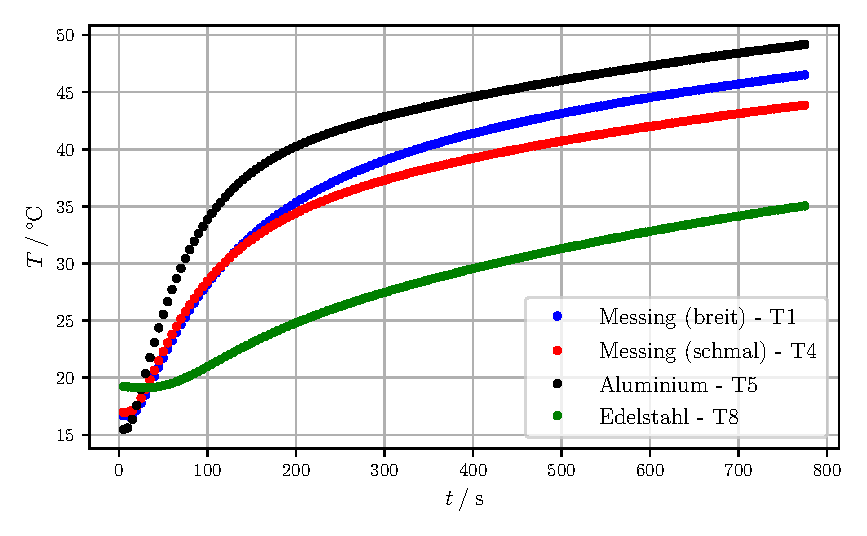
\includegraphics{build/stat_plot.pdf}
  \caption{Die Temperaturen an den fernen Messpunkte der einzelnen Stäbe bei der statischen Messung. }
  \label{fig:plot_stat}
\end{figure}
In dem Plot \autoref{fig:plot_stat} sind für die jeweiligen Stäbe die Temperaturen der vom Peltier-Element ferner liegenden Messstelle gegen die Zeit aufgetragen.
Der Aluminiumstab ist zu Anfang am kältesten mit etwas über $\SI{15}{\celsius}$, die Messingstäbe haben eine Anfangstemperatur von etwa $\SI{16}{\celsius}$, Edelstahl eine von etwa $\SI{19}{\celsius}$.
Bei allen Stäben ist ein Bereich zu erkennen, wo die Temperatur nicht ansteigt.
Für die beiden Messingstäbe und den Aluminiumstab dauert diese Phase ohne Steigung nur sehr kurz, etwa $\SI{10}{\second}$, an.
Bei Edelstahl steigt die Temperatur bis ca $t = \SI{50}{\second}$ nicht an. \\
Nach dieser Zeit steigt die Temperatur jeweils. 
Bei den Messingstäben ist die Steigung bis etwa $t=\SI{150}{\second}$ gleich, danach flacht die Steigung ab, wobei die Steigung vom breiten Messingstab etwas größer ist.
Die Temperatur vom Messingstab steigt sehr schnell an bis ca $\SI{90}{\second}$, dann nimmt die Steigung ab.
Der Edelstahlstab erwärmt sich nicht so schnell, die Steigung der Temperatur nimmt auch im weiteren Zeitverlauf ab, jedoch ist der Übergang nicht so deutlich, wie die der anderen Stäbe.
Ab dem Zeitpunkt $t=\SI{500}{\second}$ steigen die Temperaturen der Messingstäbe und des Aluminiumstabes nahezu parallel an.
Die Temperatur des Edelstahlstabes steigt noch schneller, gegen Ende der Zeitmessung scheinen alle Temperaturen der einzelnen Stäbe eine ähnliche Steigung zu haben.

Die Temperatur der jeweiligen Stäbe zum Zeitpunkt $t=\SI{700}{\second}$ lassen sich in den Messdaten ablesen und ergeben sich zu:
\begin{align*}
  \text{für den breiten Messingstab:} \: T&= \SI{45.76}{\celsius}\, =\SI{318.91}{\kelvin}\\ 
  \text{für den schmalen Messingstab:} \: T&= \SI{43.16}{\celsius}\, =\SI{316.31}{\kelvin}\\ 
  \text{für den Aluminiumstab:} \: T&= \SI{48.46}{\celsius}\, =\SI{321.61}{\kelvin}\\ 
  \text{für den Edelstahlstab:} \: T&= \SI{34.21}{\celsius}\, =\SI{307.36}{\kelvin}
\end{align*}

Nach der Gleichung \eqref{eqn:Wärmemenge} lässt sich der Wärmestrom $\frac{\Delta Q}{\Delta t}$ für die verschiedenen Metallstäbe errechnen (siehe Tabelle \ref{tab:Wärmestrom}).
Dabei wird für das $\kappa $ der Wert aus der Literatur genommen (siehe Vorbereitung \ref{tab:}) und der Abstand $x$ der Tempertaurmessstellen wurde zu $x = \SI{3}{\centi\metre}$ nachgemessen.
\begin{table}
  \centering
  \caption{Der Wärmestrom der verschiedenen Metallstäben zu 5 verschiedenen Zeitpunkten.}
  \label{tab:Wärmestrom}
  \begin{tabular}{S[table-format=3.0] %Zeit
                  S[table-format=1.3] %Messing breit
                  S[table-format=1.3] %Messing schmal
                  S[table-format=1.3] %ALuminium
                  S[table-format=1.3] %Edelstahl
                  }
  \toprule
  &\multicolumn{4}{c}{$\frac{\Delta Q}{\Delta t} [\si{\joule\per\second}]$}\\
  \cmidrule(lr){2-5}
  {$ t [\si{\second}]$}&{Messing (breit)}&{Messing (schmal)}&{Aluminium}&{Edelstahl}\\
  \midrule
  100 & 1.150 & 0.794 & 1.422 & 0.286 \\
  200 & 0.726 & 0.548 & 0.838 & 0.285 \\
  350 & 0.518 & 0.451 & 0.641 & 0.260 \\
  450 & 0.474 & 0.435 & 0.611 & 0.252 \\
  600 & 0.447 & 0.428 & 0.595 & 0.245 \\
  \bottomrule
  \end{tabular}
\end{table}
Abschließend werden die Temperaturdifferenzen zwischen den Temperaturmessstellen eines Stabes für den breiten Messingstab und den Edelstahlstab in einem $t$-$T$- Diagramm aufgetragen.
\begin{figure}[H]
  \centering
  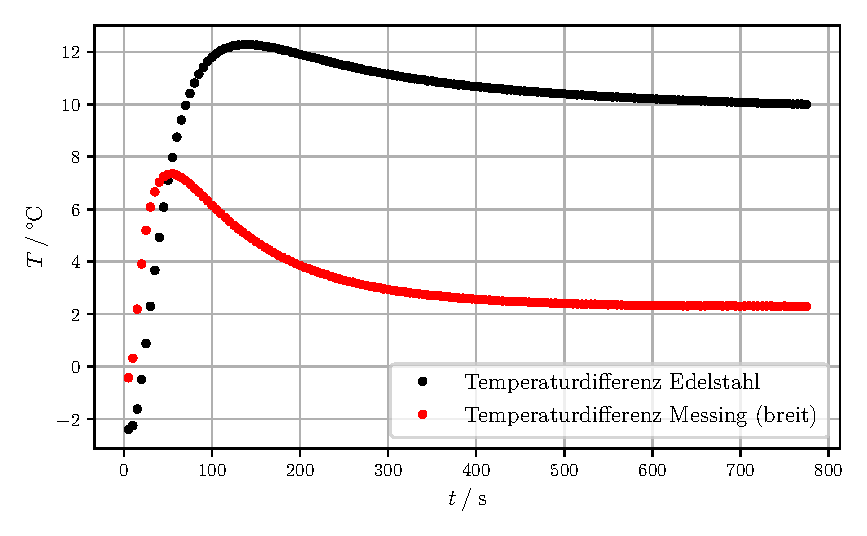
\includegraphics[width=\textwidth]{build/plot_diff.pdf}
  \caption{Die Temperaturdifferenzen zwischen den Messstellen auf einem Stab.}
  \label{fig:plot_diff}
\end{figure}
In der \autoref{fig:plot_diff} fällt auf, dass bei beiden Stoffen der Temperaturunterschied im Negativen startet und dann stark ansteigt.
Die Temperaturdifferenz innerhalb des breiten Messingstabes hat bei etwa $ t = \SI{50}{\second}$ seinen Hochpunkt von $\SI{7.5}{\celsius}$ erreicht.
Dann fällt die Kurve, flacht ab und nähert sich einem Wert um die $\SI{2}{\celsius}$ an.
Die Temperaturdifferenz des Edelstahlstabes steigt höher als die des breiten Messingstabes bis sie ihren Hochpunkt bei etwa $\SI{120}{\second} $ und $\SI{12.2}{\celsius}$ erreicht hat.
Die Kurve fällt daraufhin flach ab und bis zum Ende der Aufnahme wird die negative Steigung immer kleiner.

\subsection{Dynamische Methode}
In der dynamische Methode wurden die Stäbe in periodischen Abständen gewärmt und gekühlt. 
Für die Auswertung von den breiten Messingstab und dem Aluminiumstab beträgt die Periode $\SI{80}{\second}$.
Es wurden alle $\SI{2}{\second}$ die Temperatur jedes Stabes an zwei Stellen mit einem Abstand von $\SI{3}{\centi\metre}$ aufgenommen. 


\subsubsection{Messingstab (breit)}
Es wird zuerst der breite Messingstab betrachtet. 
In der Abbildung \ref{fig:messing_dyn} sind die beiden Temperaturverläufe der einzelnen Messstellen gegen die Zeit aufgetragen.
\begin{figure}[H]
  \centering
  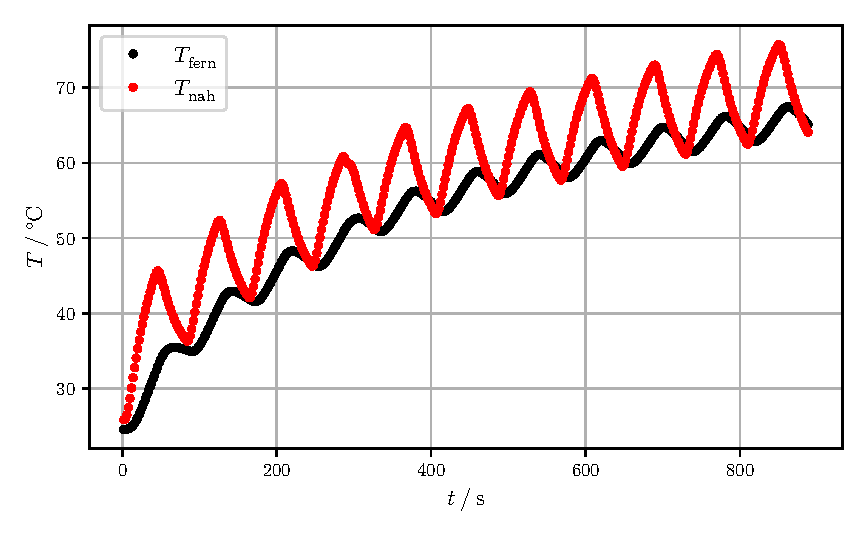
\includegraphics{build/plot_messing.pdf}
  \caption{Die Temperaturen an den verschiedenen Messstellen des Messingstabes in der dynamischen Methode mit einer Periode von $\SI{80}{\second}$.}
  \label{fig:messing_dyn}
\end{figure}
Es ist in der \autoref{fig:messing_dyn} eindeutig die Periodizität der Messung zu sehen.
Auffällig ist der stärkere Amplituden an der Messstelle, die nah an dem Peltier-Element liegt.
Auch der Phasenunterschied $\Delta t$ ist erkennbar.\\
\\
Die Amplituden und deren Phasendifferenz sind in der Tabelle \ref{tab:messing_dyn} aufgelistet.
Es ergibt sich aus den Werten der Mittelwert:
\begin{align*}
  ln(\frac{A_{\text{nah}}}{A_{\text{fern}}}) &= \num{0.904 \pm 0.013}\\
  \Delta t &= \SI{14.545 \pm 0.311}{\second}
\end{align*} 

\begin{table}
  \centering
  \caption{Die Amplituden und Phasendifferenz des Messingstabes.}
  \label{tab:messing_dyn}
  \begin{tabular}{S[table-format=2.2] %A nah
                  S[table-format=2.2] % A fern
                  S[table-format=1.3] % ln
                  S[table-format=2]}
  \toprule
  {$ A_{\text{nah}} [\si{\kelvin}] $}&
  {$ A_{\text{fern}} [\si{\kelvin}] $}&
  {$ \log(\frac{A_{\text{nah}}}{A_{\text{fern}}})$} &
  {$ \Delta t [\si{\second}]$}\\
  \midrule
  19.81  &10.93 & 0.595& 22\\
  16.07  &  8.01 & 0.696& 16\\
  15.17  &  6.77 & 0.807& 16\\
  14.58  &  6.43 & 0.819& 20\\
  13.55  &  5.38 & 0.924& 14\\
  13.98  &  5.29 & 0.972& 12\\
  13.76  &  5.11 & 0.991& 12\\
  13.55  &  4.92 & 1.013& 12\\
  13.46  &  4.85 & 1.021& 12\\
  13.27  &  4.65 & 1.049& 12\\
  13.26  &  4.59 & 1.061& 12\\
  \bottomrule
  \end{tabular}
\end{table}
Nach der Gleichung \eqref{eqn:kappa}
kann nun die Wärmeleitfähigikeit berechnet werden:
\begin{equation*}
  \kappa = \SI{117.264 \pm 0.937}{\watt\per\metre\kelvin}
\end{equation*}
Für die Temperaturwelle lassen sich daraus die Frequenz $f$ und die Wellenlänge $\lambda $ berechnen.
Es wurde die Formel in \eqref{eqn:lambda} benutzt.
\begin{align*}
  f &= \frac{1}{T} = \SI{0.0125}{\hertz}\\
  \lambda &= \SI{0.189 \pm 0.003}{\metre}
\end{align*}

\subsubsection{Aluminiumstab}
Für den Aluminiumstab wird das Vorgehen wiederholt.
Die Temperatur des Aluminiumstab wurde an zwei Messstelle alle $\SI{2}{\second}$ aufgeschrieben.
Die Temperaturen der einzelnen Stellen wurden gegen die Zeit in ein Diagramm aufgetragen.
\begin{figure}[H]
  \centering
  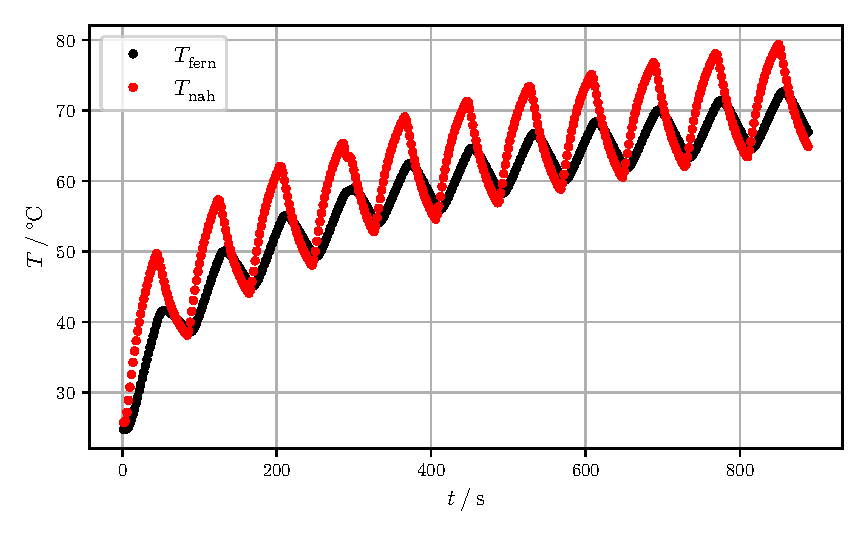
\includegraphics{build/plot_aluminium.pdf}
  \caption{Die Temperaturen an den einzelnen Messstellen des Aluminiumstabes bei der dynamischen Methode mit $T=\SI{80}{\second}$.}
  \label{fig:aluminium_dyn}
\end{figure}
In der \autoref{fig:aluminium_dyn} sind die periodischen Verläufe der Temperatur zu erkennen, sowie der Phasenunterschied der Amplituden.
Die Temperatur, die an der Messstelle, die nah an dem Peltier-Element liegt, gemessen wurde, hat eine größeren Ausschlag, als die Temperatur, die weiter vom Peltier-Element weg gemessen wurde.
\\
\\
Die Amplituden der Temperaturverläufe und die Phasendifferenz $\Delta t$ werden für die weiteren Berechnungen benötigt.
\begin{table}
  \centering
  \caption{Die Amplituden und Phasendifferenz der Temperaturmessungen am Aluminiumstab.}
  \label{tab:aluminium_dyn}
  \begin{tabular}{
    S[table-format=2.2] %A nah
    S[table-format=2.2] % A fern
    S[table-format=1.3] % ln
    S[table-format=2]}
  \toprule
  {$ A_{\text{nah}} [\si{\kelvin}] $}&
  {$ A_{\text{fern}}[\si{\kelvin}] $}&
  {$ \log(\frac{A_{\text{nah}}}{A_{\text{fern}}})$} &
  {$ \Delta t [\si{\second}]$}\\
  \midrule
  23.96 & 16.91  & 0.348  & 12\\
  19.19 & 11.49  & 0.513  & 8\\
  17.96 & 10.01  & 0.585  & 8\\
  17.27 & 9.59  & 0.588  & 14\\
  16.25 & 8.42  & 0.657  & 6\\
  16.71 & 8.66  & 0.657  & 8\\
  16.43 & 8.51  & 0.658  & 6\\
  16.23 & 8.28  & 0.673  & 6 \\
  16.22 & 8.23  & 0.678  & 6\\
  16.01 & 8.08  & 0.684  & 8\\
  15.9  & 8.06  & 0.679  & 6\\
  \bottomrule  
  \end{tabular}
\end{table}
Aus den Daten in der Tabelle \ref{tab:aluminium_dyn} sind die folgende Werte festgelegt:
\begin{align*}
  \log(\frac{A_{\text{nah}}}{A_{\text{fern}}}) &= \num{0.611 \pm 0.009}\\
  \Delta t &= \SI{8.0 \pm 0.233}{\second}
\end{align*}
Nach der Gleichung \eqref{eqn:kappa} lässt sich nun die Wärmeleitfähigkeit $\kappa $ berechnen:
\begin{equation*}
  \kappa = \SI{231.646 \pm 3.763}{\watt\per\metre\kelvin}
\end{equation*}
Die Frequenz $f$ und die Wellenlänge $\lambda$ ergeben sich nach \eqref{eqn:lambda} schließlich zu:
\begin{align*}
  f &= \SI{0.0125}{\hertz}\\
  \lambda &= \SI{0.315 \pm 0.003}{\metre}
\end{align*}

\subsubsection{Edelstahlstab}
Für die Auswertung des Edelstahlstabes werden Messdaten von einer anderen dynamischen Messung mit einer Periode von $T = \SI{200}{\second}$ betrachtet.
Es wurden wieder die Temperaturen an zwei verschiedenen Messstellen des Edelstahlstabes mit Abstand $\Delta x = \SI{3}{\centi\metre}$ alle $ \SI{2}{\second}$ gemessen.\\
\\
Die Temperaturverläufe werde in einem $t$-$T$- Diagramm abgebildet. 
In der \autoref{fig:edelstahl_dyn} sind die periodischen Veränderungen der Temperaturen deutlich zu erkennen.
Die Temperatur, die nah an dem Peltier-Element gemessen wurde, zeigt einen zeitlich früher einen größeren Ausschlag, als die weiter vom Peltier-Element entfernt gemessenen Temperatur.
Die verschiedenen Amplitudenausschläge und deren Phasendifferenz $\Delta t$ sind in der Tabelle \ref{tab:edelstahl_dyn} zu finden. 
\begin{figure}
  \centering
  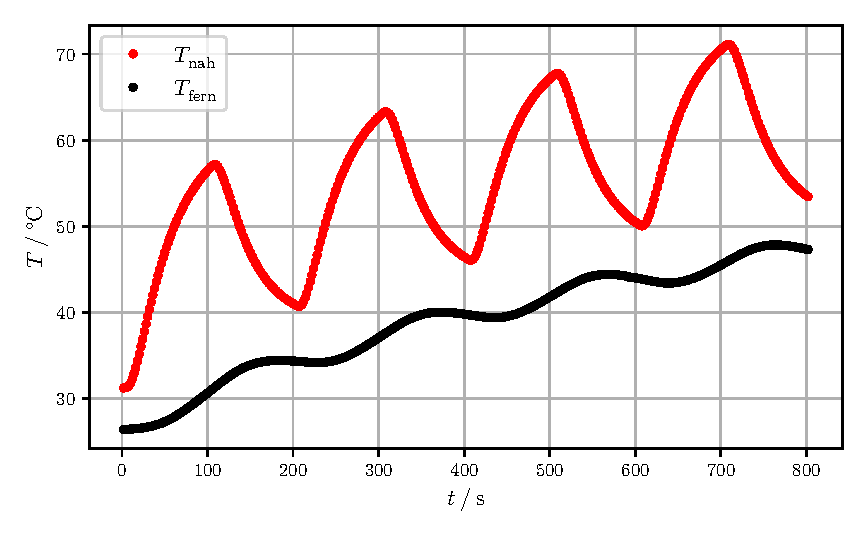
\includegraphics{build/plot_edelstahl.pdf}
  \caption{Die Temperaturen der verschiedenen Messstellen des Edelstahlstabes.}
  \label{fig:edelstahl_dyn}
\end{figure}

\begin{table}
  \centering
  \caption{Die Amplituden und Phasendifferenz beim Edelstahlstab.}
  \label{tab:edelstahl_dyn}
  \begin{tabular}{S[table-format=2.2]
                  S[table-format=2.2]
                  S[table-format=1.3]
                  S[table-format=2]}
  \toprule
  {$ A_{\text{nah}} [\si{\kelvin}] $}&
  {$ A_{\text{fern}} [\si{\kelvin}] $}&
  {$ \log(\frac{A_{\text{nah}}}{A_{\text{fern}}})$} &
  {$ \Delta t [\si{\second}]$}\\
  \midrule
  25.97 & 8.02 & 1.175 & 76\\
  22.58 & 5.85 & 1.351 & 66\\
  21.72 & 5.01 & 1.467 & 62\\
  21.07 & 4.42 & 1.562 & 56\\
  \bottomrule  
  \end{tabular}
\end{table}
Aus den Daten in Tabelle \ref{tab:edelstahl_dyn} ergeben sich folgende Mittelwerte:
\begin{align*}
  ln(\frac{A_{\text{nah}}}{A_{\text{fern}}}) &= \num{1.389 \pm 0.036}\\
  \Delta t &= \SI{65.0 \pm 1.82}{\second}
\end{align*}
Letztlich berechnet sich die Wärmeleitfähigkeit nach der Gleichung \eqref{eqn:kappa} für Edelstahl zu:
\begin{equation*}
  \kappa = \SI{16.145 \pm 0.056}{\watt\per\metre\per\kelvin}
\end{equation*}
Die Temperaturwelle hat demnach, berechnet mit der Gleichung \eqref{eqn:lambda} die Frequenz $f$ und die Wellenlänge $\lambda$ mit den Werten:
\begin{align*}
  f &= \SI{0.005}{\hertz}\\
  \lambda &= \SI{7.122(12)e-2}{\metre}
\end{align*}